\documentclass{article}
\usepackage[margin=0.75in]{geometry}
\usepackage{booktabs}
\usepackage{caption}
\usepackage{graphicx}
\usepackage{float}
\graphicspath{ {./Images/} }

\title{Trading Strategies Summary}
\author{Varun Varanasi}

\begin{document}
\maketitle

The goal of this document is to outline different trading strategies implemented with the Metaculus data on the VIX, SPY, and their derivatives. Each strategy only trades 1 stock per action and was optimized for the maximal Sharpe Ratio.

\section*{Metaculus Momentum}
This simple strategy involves opening a position when the Metaculus series increases and closing the position when it decreases. This strategy only allows for one open position at a time.

\begin{table}[h]
\centering

\begin{tabular}{l||ccc}
    \toprule
     & \textbf{VXX} & \textbf{SPY} & \\
    \midrule
    PnL & \$38.10 & \$86.85 \\
    Sharpe Ratio & -2.06 & -4.89\\
    Percent Underwater & 6\% & 27\%\\
    \bottomrule
\end{tabular}
\caption{Summary of results from 1/1/2020 to 4/1/2022}
\end{table}

\begin{figure}[H]
\centering
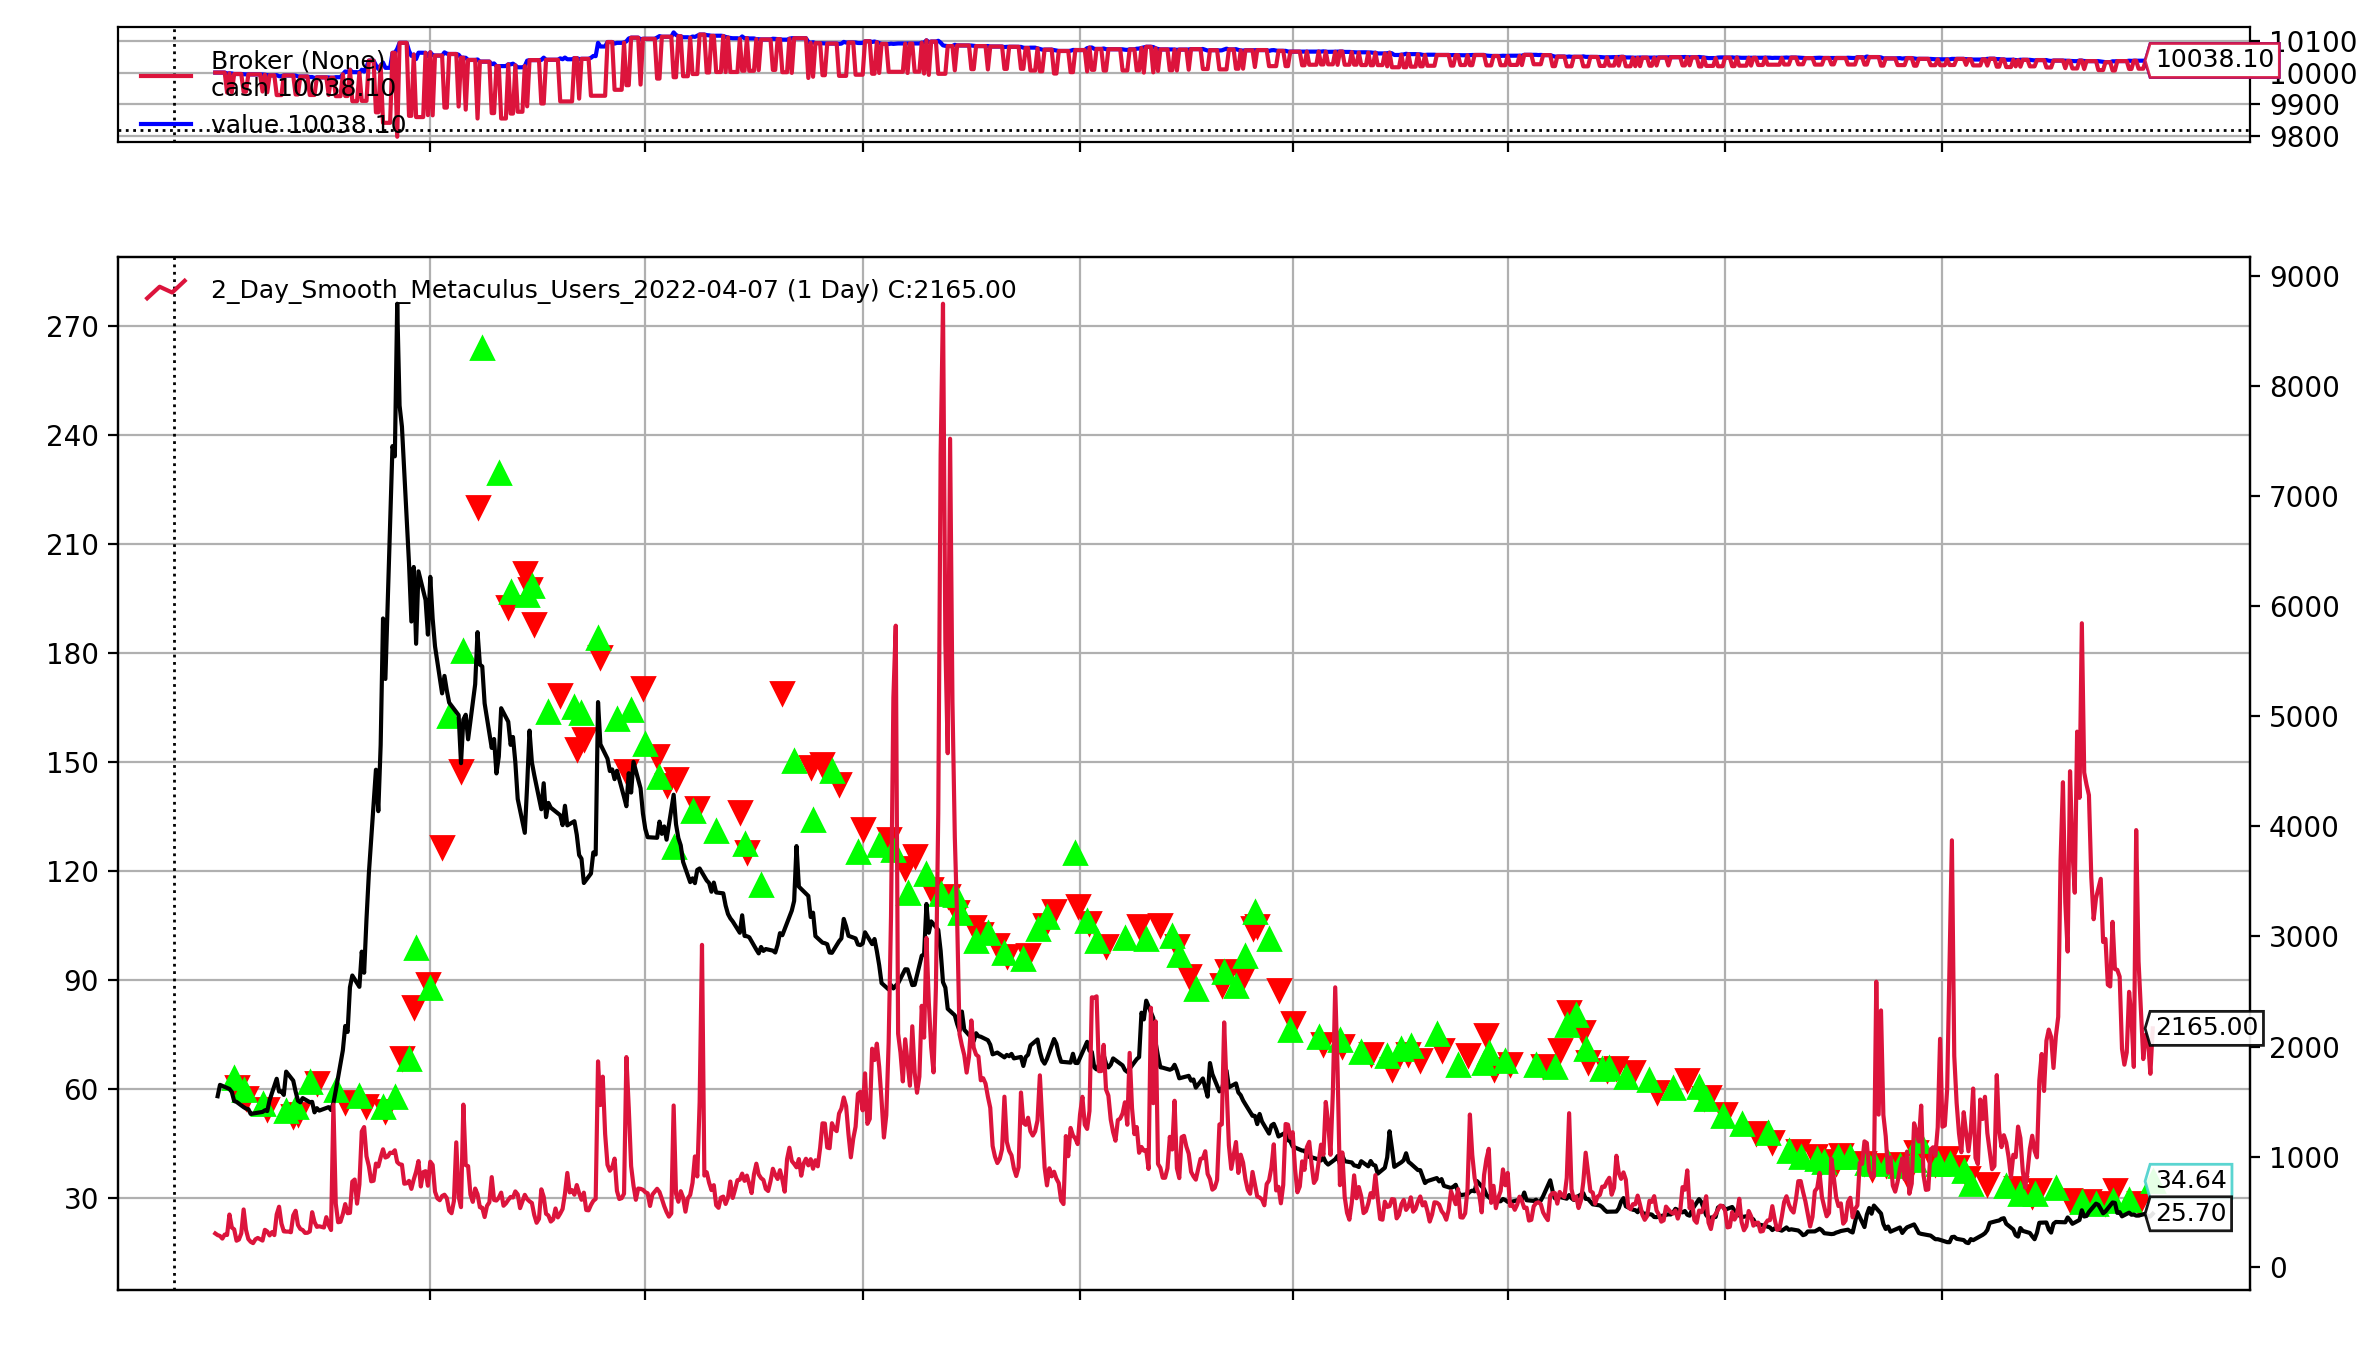
\includegraphics[width=\textwidth]{Metaculus_Momentum_VXX.png}
\caption{VXX and Metaculus Trading Plot}
\end{figure}

\begin{figure}[H]
    \centering
    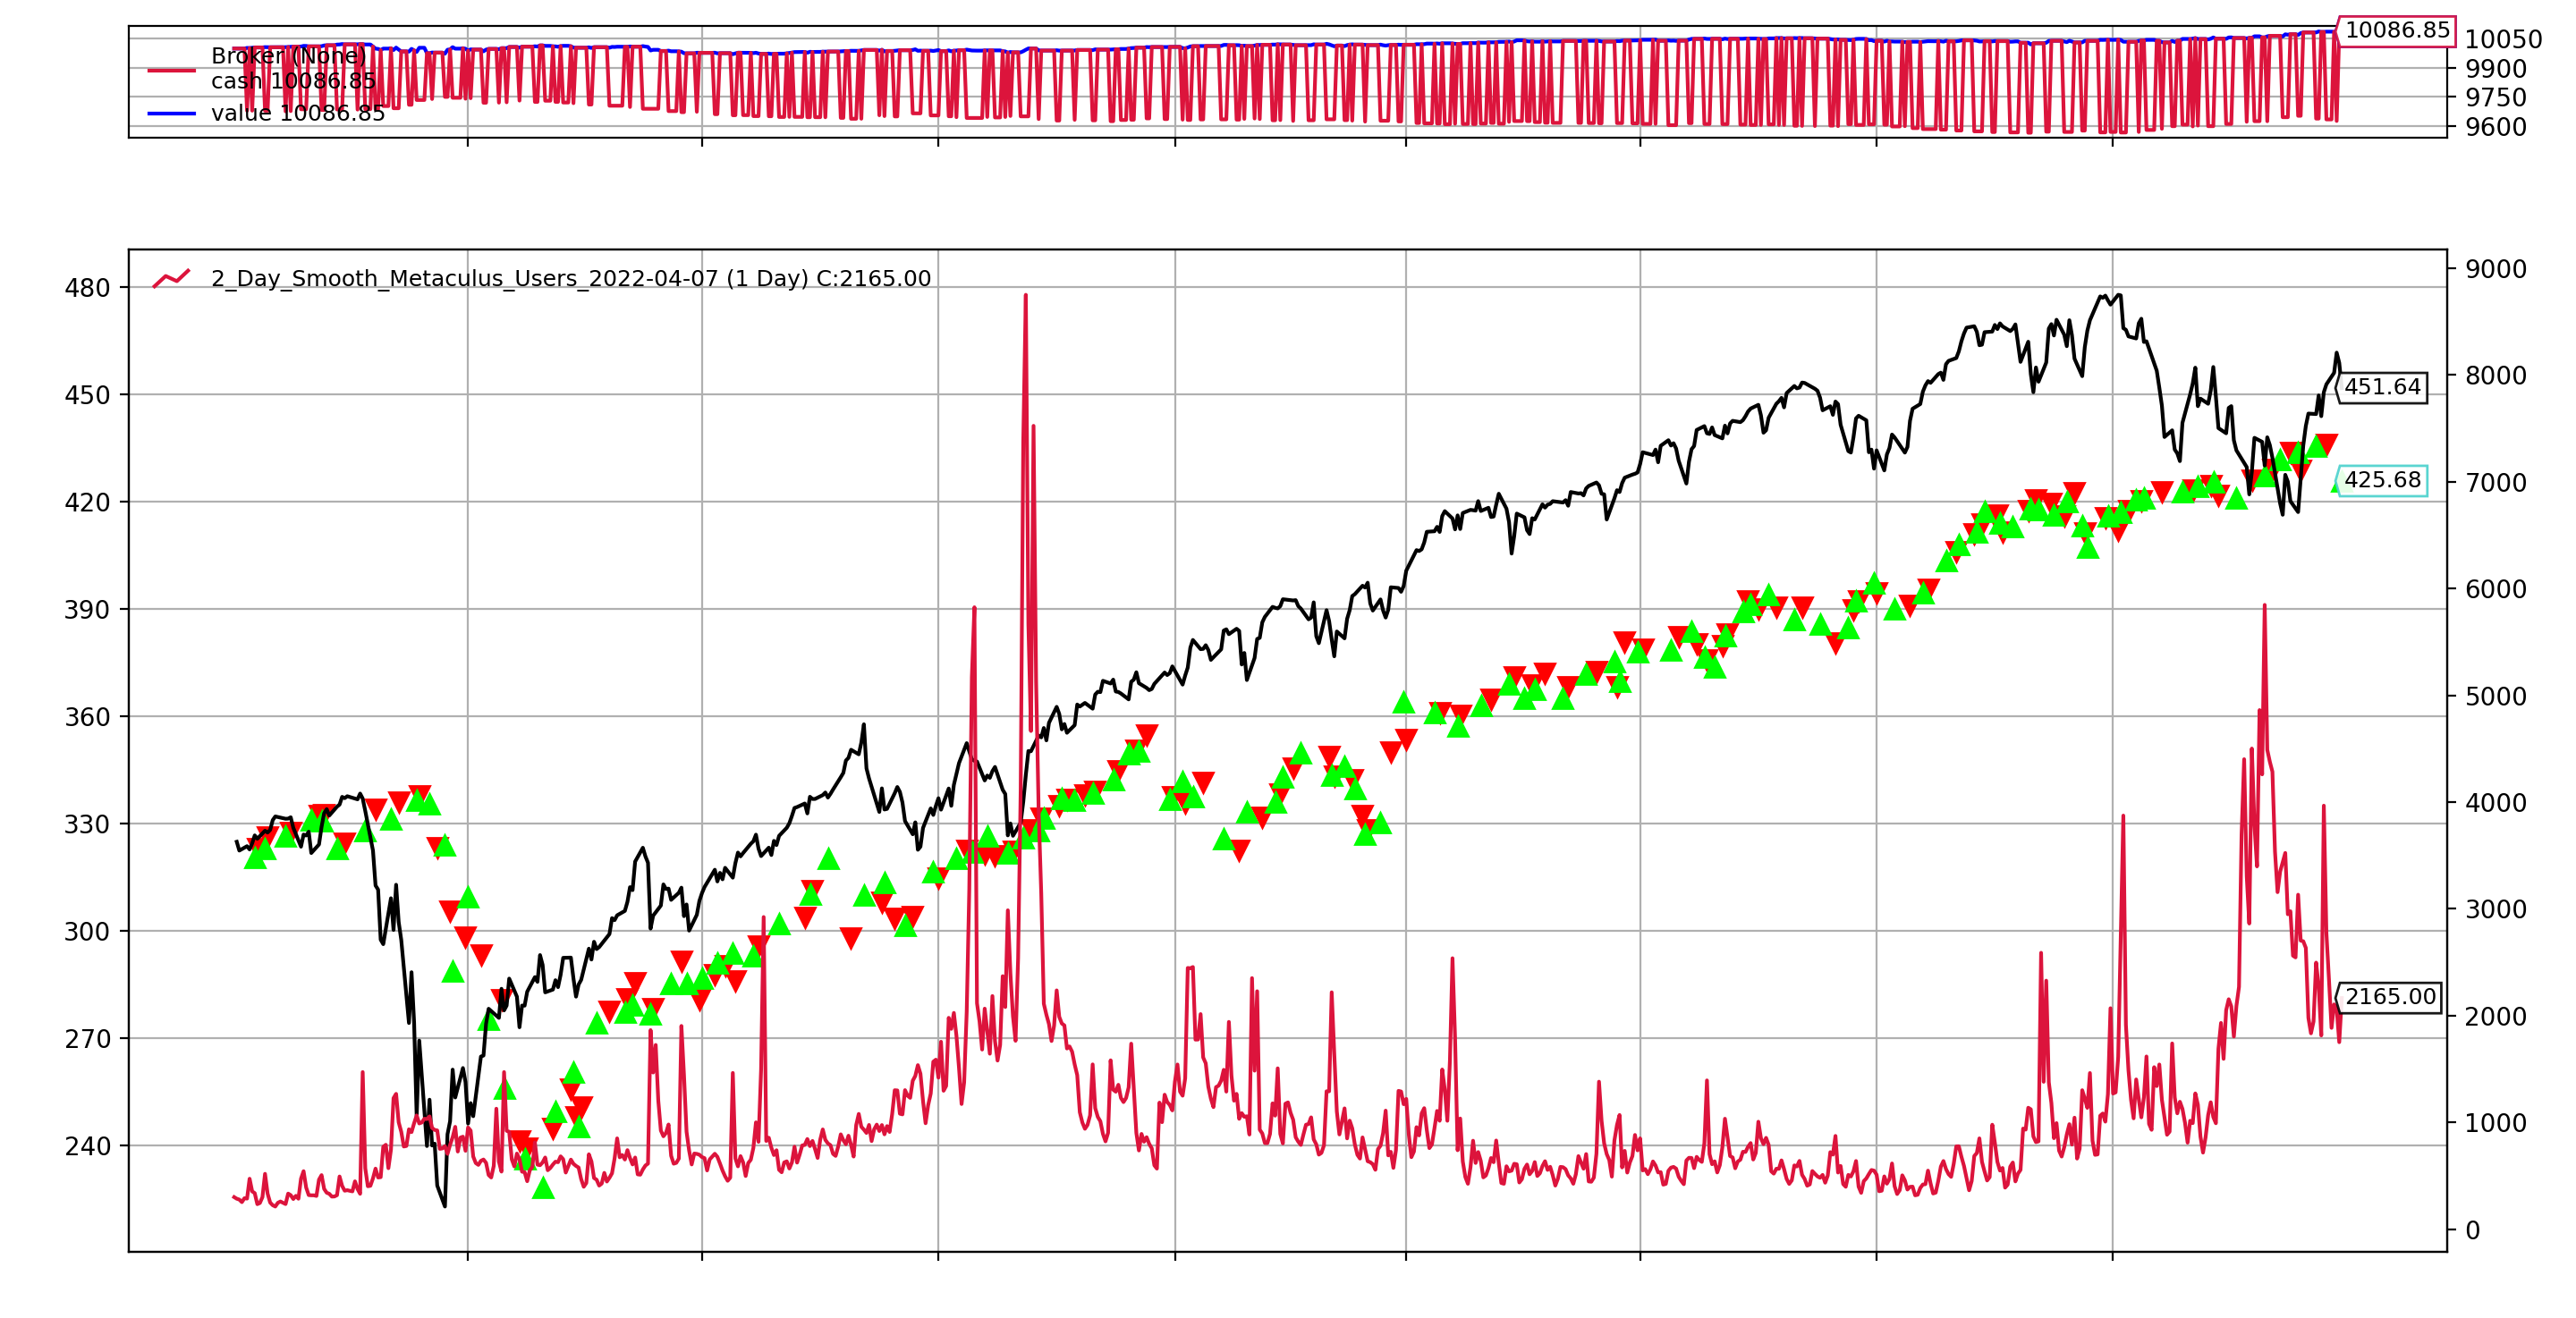
\includegraphics[width=\textwidth]{Metaculus_Momentum_SPY.png}
    \caption{SPY and Metaculus Trading Plot}
\end{figure}

\newpage

\section*{Metaculus Moving Average}
This strategy involves a slow and a fast moving average indicator on the Metaculus series. For the SPY, when the fast moving average passes the slow moving average (indicating populace uncertainity), we short as we expect volatility to increase. We then close our positions when the slow moving average passes the fast one.
Similarly, for the VXX, we trade using the opposite strategy. The fast moving average passing the slow one is interpretted as a signal to buy while the slow passing the fast is a signal to close the position. In both cases, if the position is open for a pre-determined hold period, it is immediately closed. We ran optimization on the slow, fast, and hold-periods to find the following results:

\begin{table}[h]
    \centering
    
    \begin{tabular}{l||ccc}
        \toprule
         & \textbf{VXX} & \textbf{SPY} & \\
        \midrule
        Slow Moving Average & 66  & 50\\
        Fast Moving Average & 10  & 16\\
        Hold Period & 16  & 19\\
        PnL & \$132.35 & \$96.30 \\
        Sharpe Ratio & -1.16 & -1.20\\
        Percent Underwater & 1\% &  0\%\\
        \bottomrule
    \end{tabular}
    \caption{Summary of results from 1/1/2020 to 4/1/2022}
    \end{table}

\begin{figure}[H]
\centering
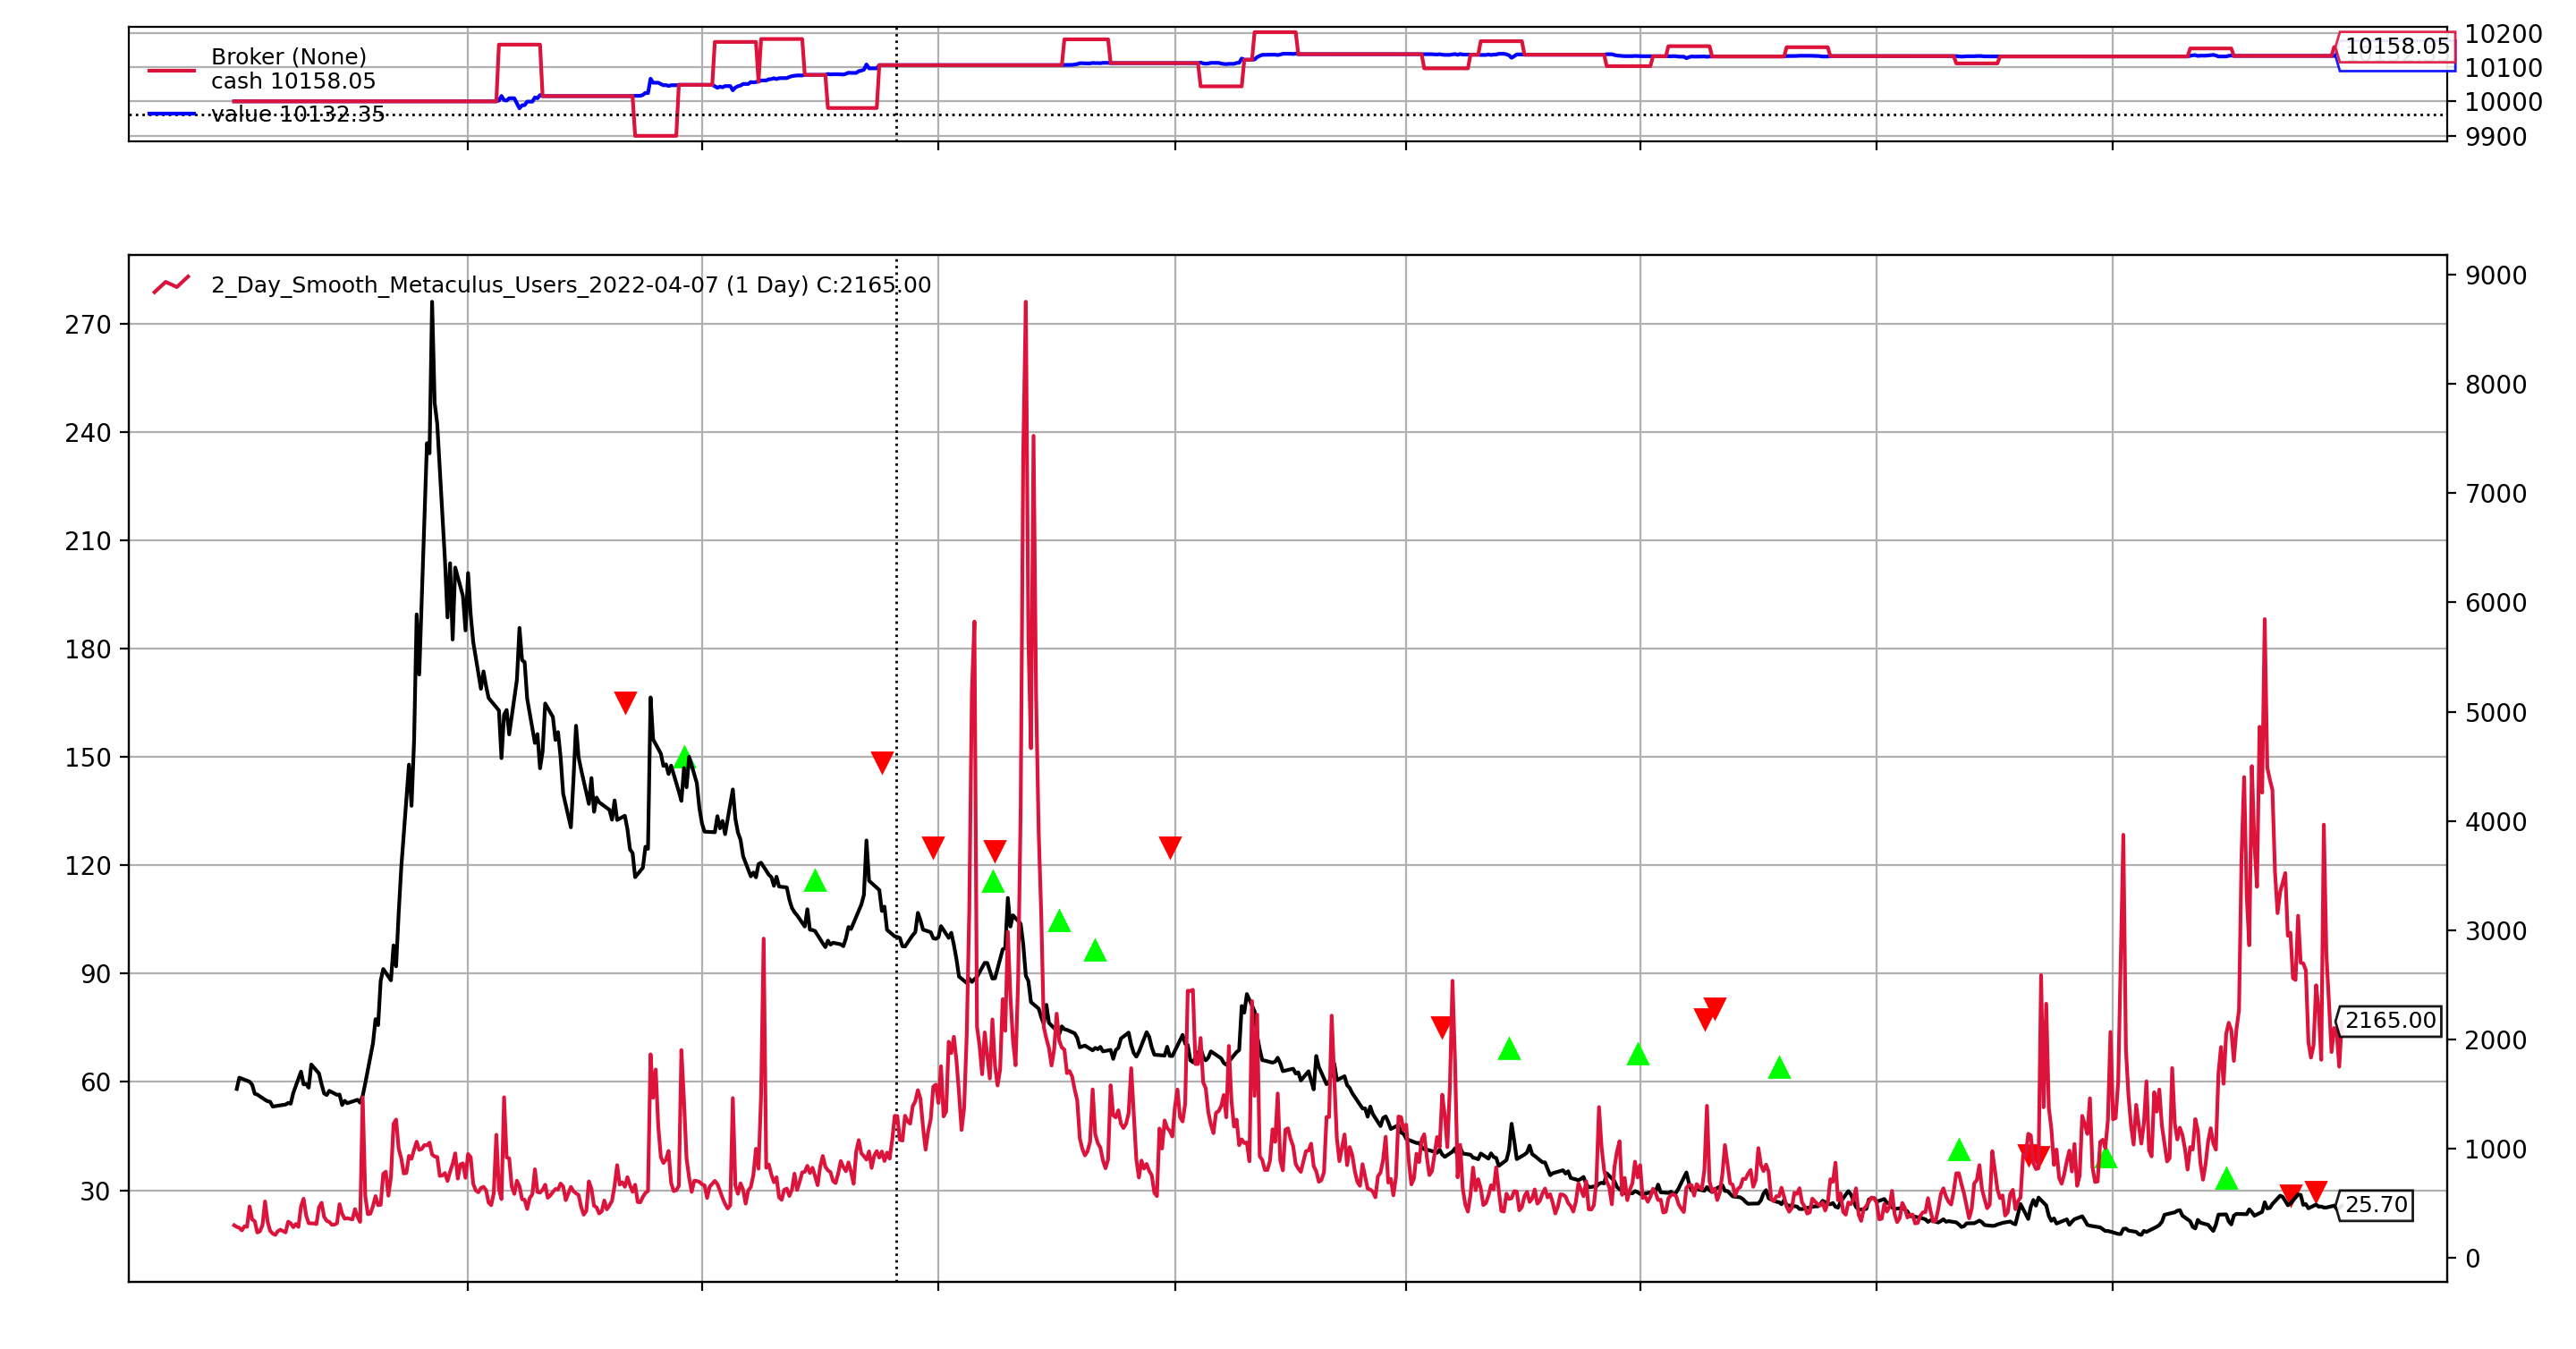
\includegraphics[width=\textwidth]{Metaculus_MA_VXX.png}
\caption{VXX and Metaculus Trading Plot}
\end{figure}
        
\begin{figure}[H]
\centering
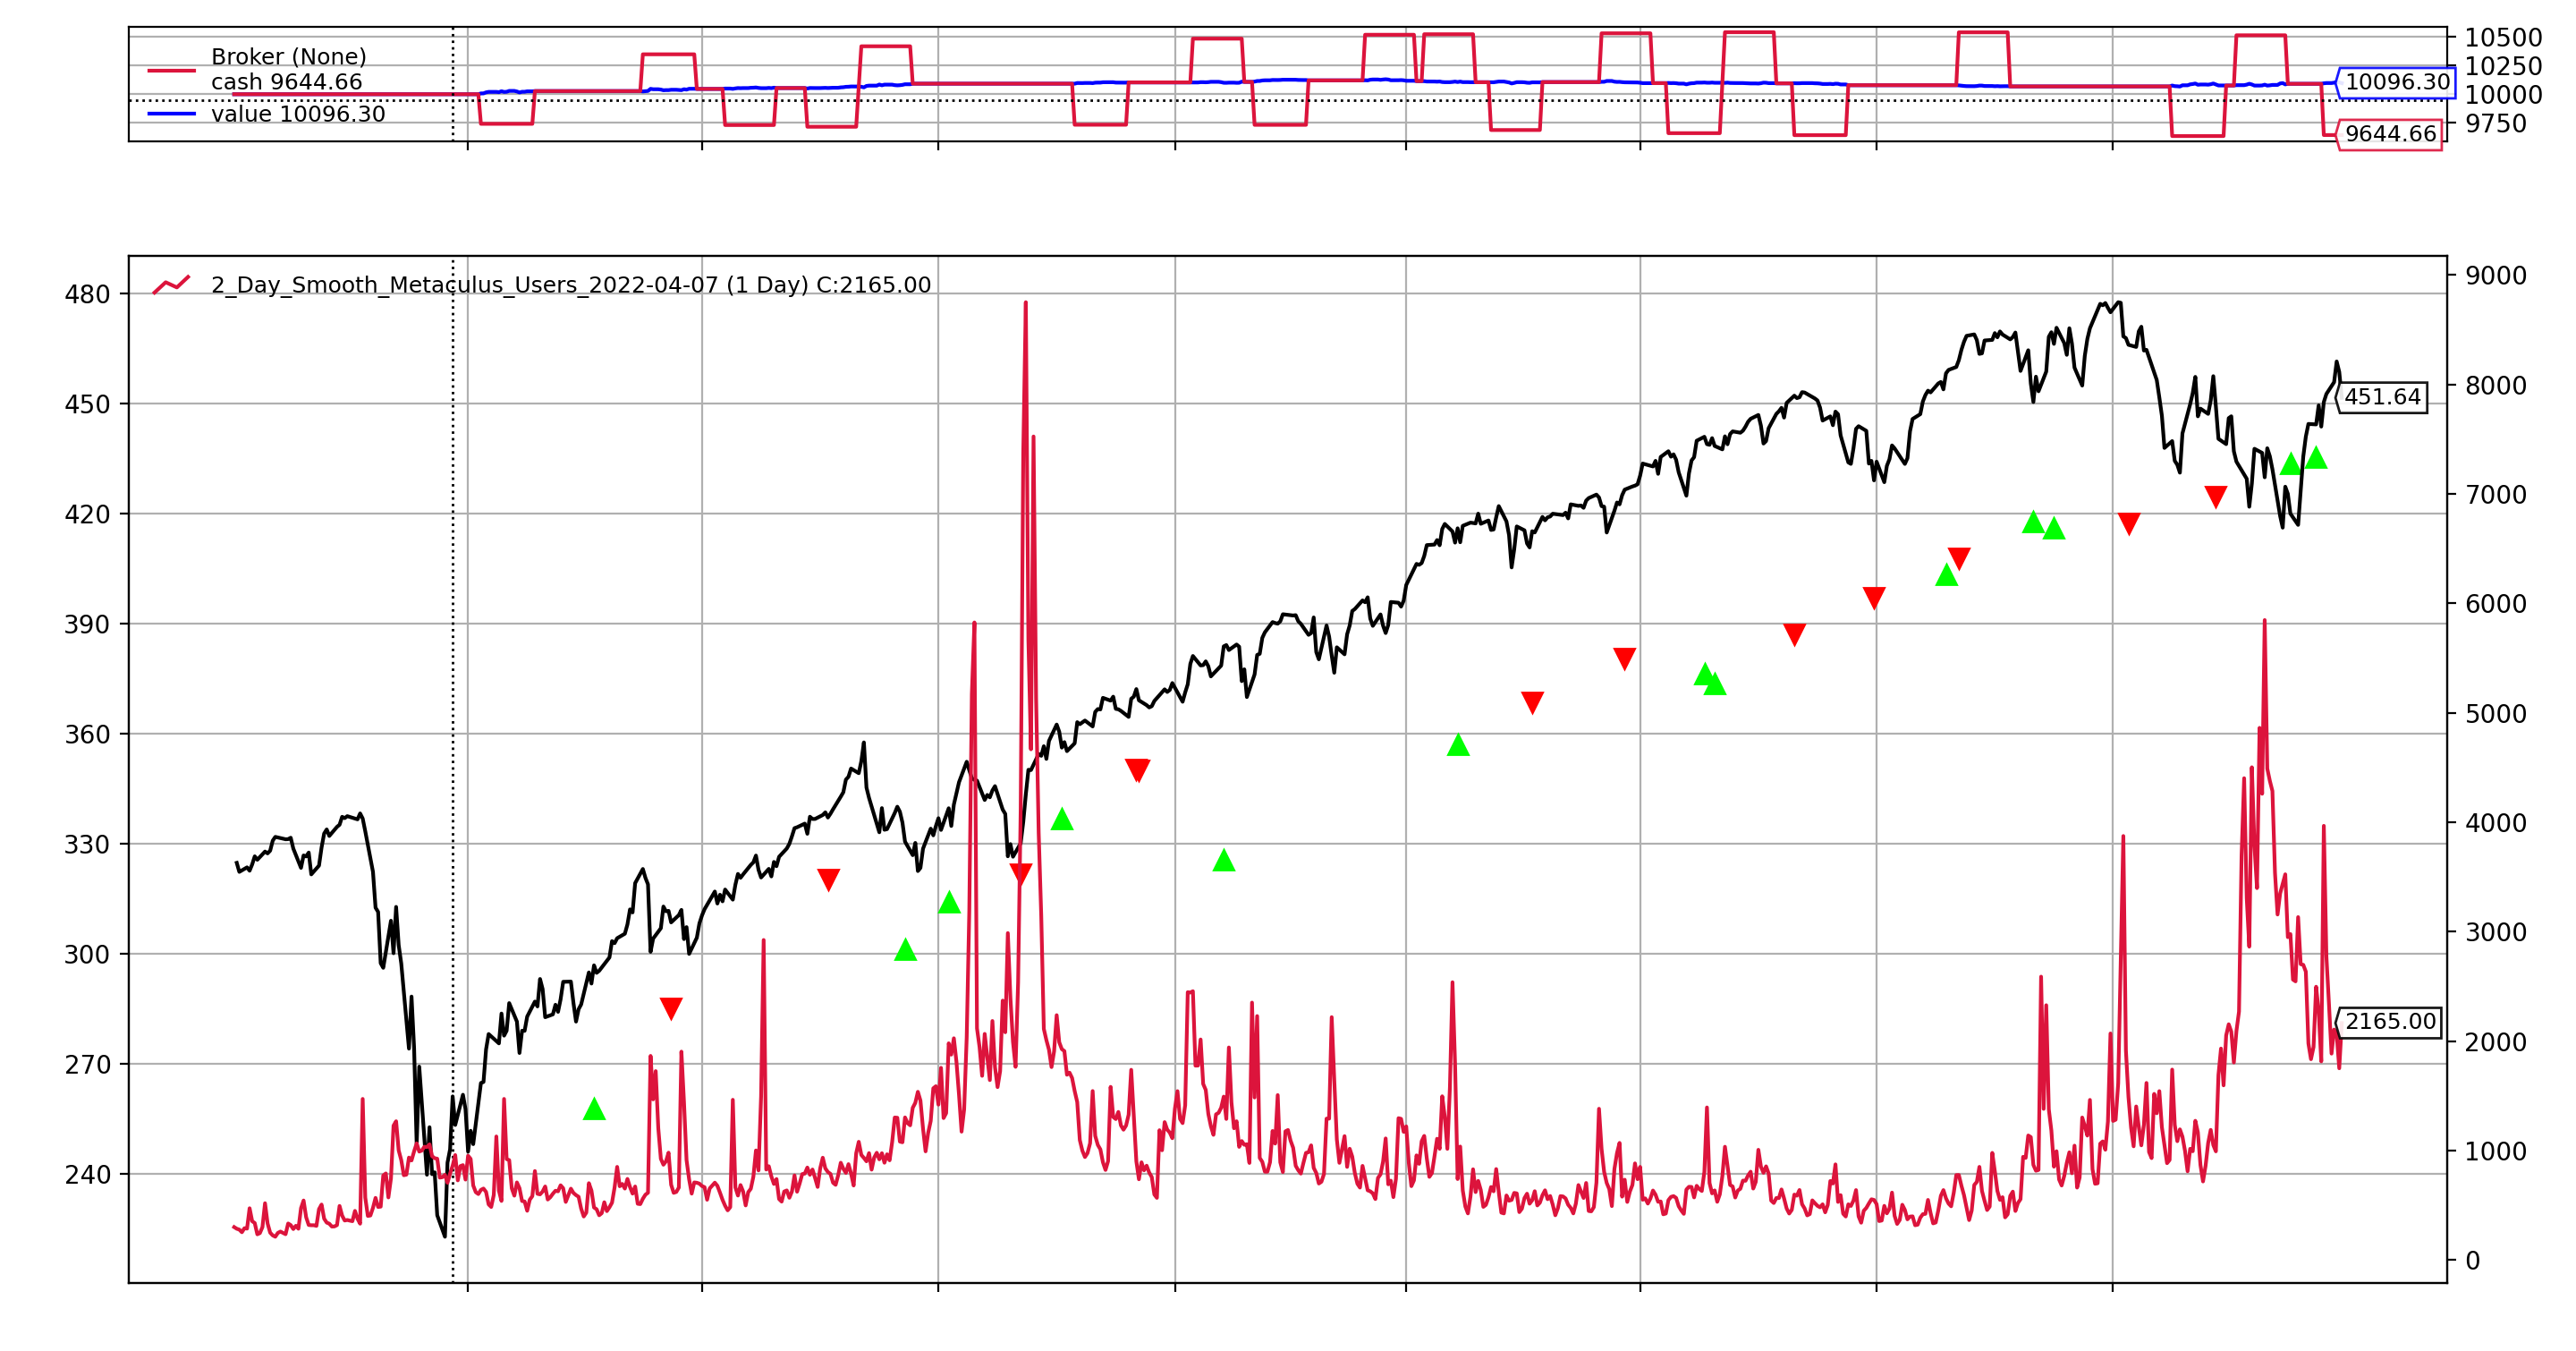
\includegraphics[width=\textwidth]{Metaculus_MA_SPY.png}
\caption{SPY and Metaculus Trading Plot}
\end{figure}
    

\newpage

\section*{Metaculus Lead}
This strategy involves monitoring the percent change over the course of 5 days in Metaculus user data. If the percent increase of users surpasses a pre-determined threshold, the strategy will opens a position number of days later.  This position is then closed once the metaculus user data drops by at least the pre-determined threshold. Optimization tests on the percent change threshold and leading period yielded the following results:

\begin{table}[h]   
    \centering
    \begin{tabular}{l||ccc}
        \toprule
        & \textbf{VXX} & \textbf{SPY} & \\
        \midrule
        Lag & 11  & 21\\
        Threshold & 20\%  & 50\%\\
        PnL & \$252.20 & \$152.79 \\
        Sharpe Ratio & -0.12 & -0.77\\
        Percent Underwater & 0\% &  8\%\\
        \bottomrule
    \end{tabular}
    \caption{Summary of results from 1/1/2020 to 4/1/2022}
\end{table}

\begin{figure}[H]
    \centering
    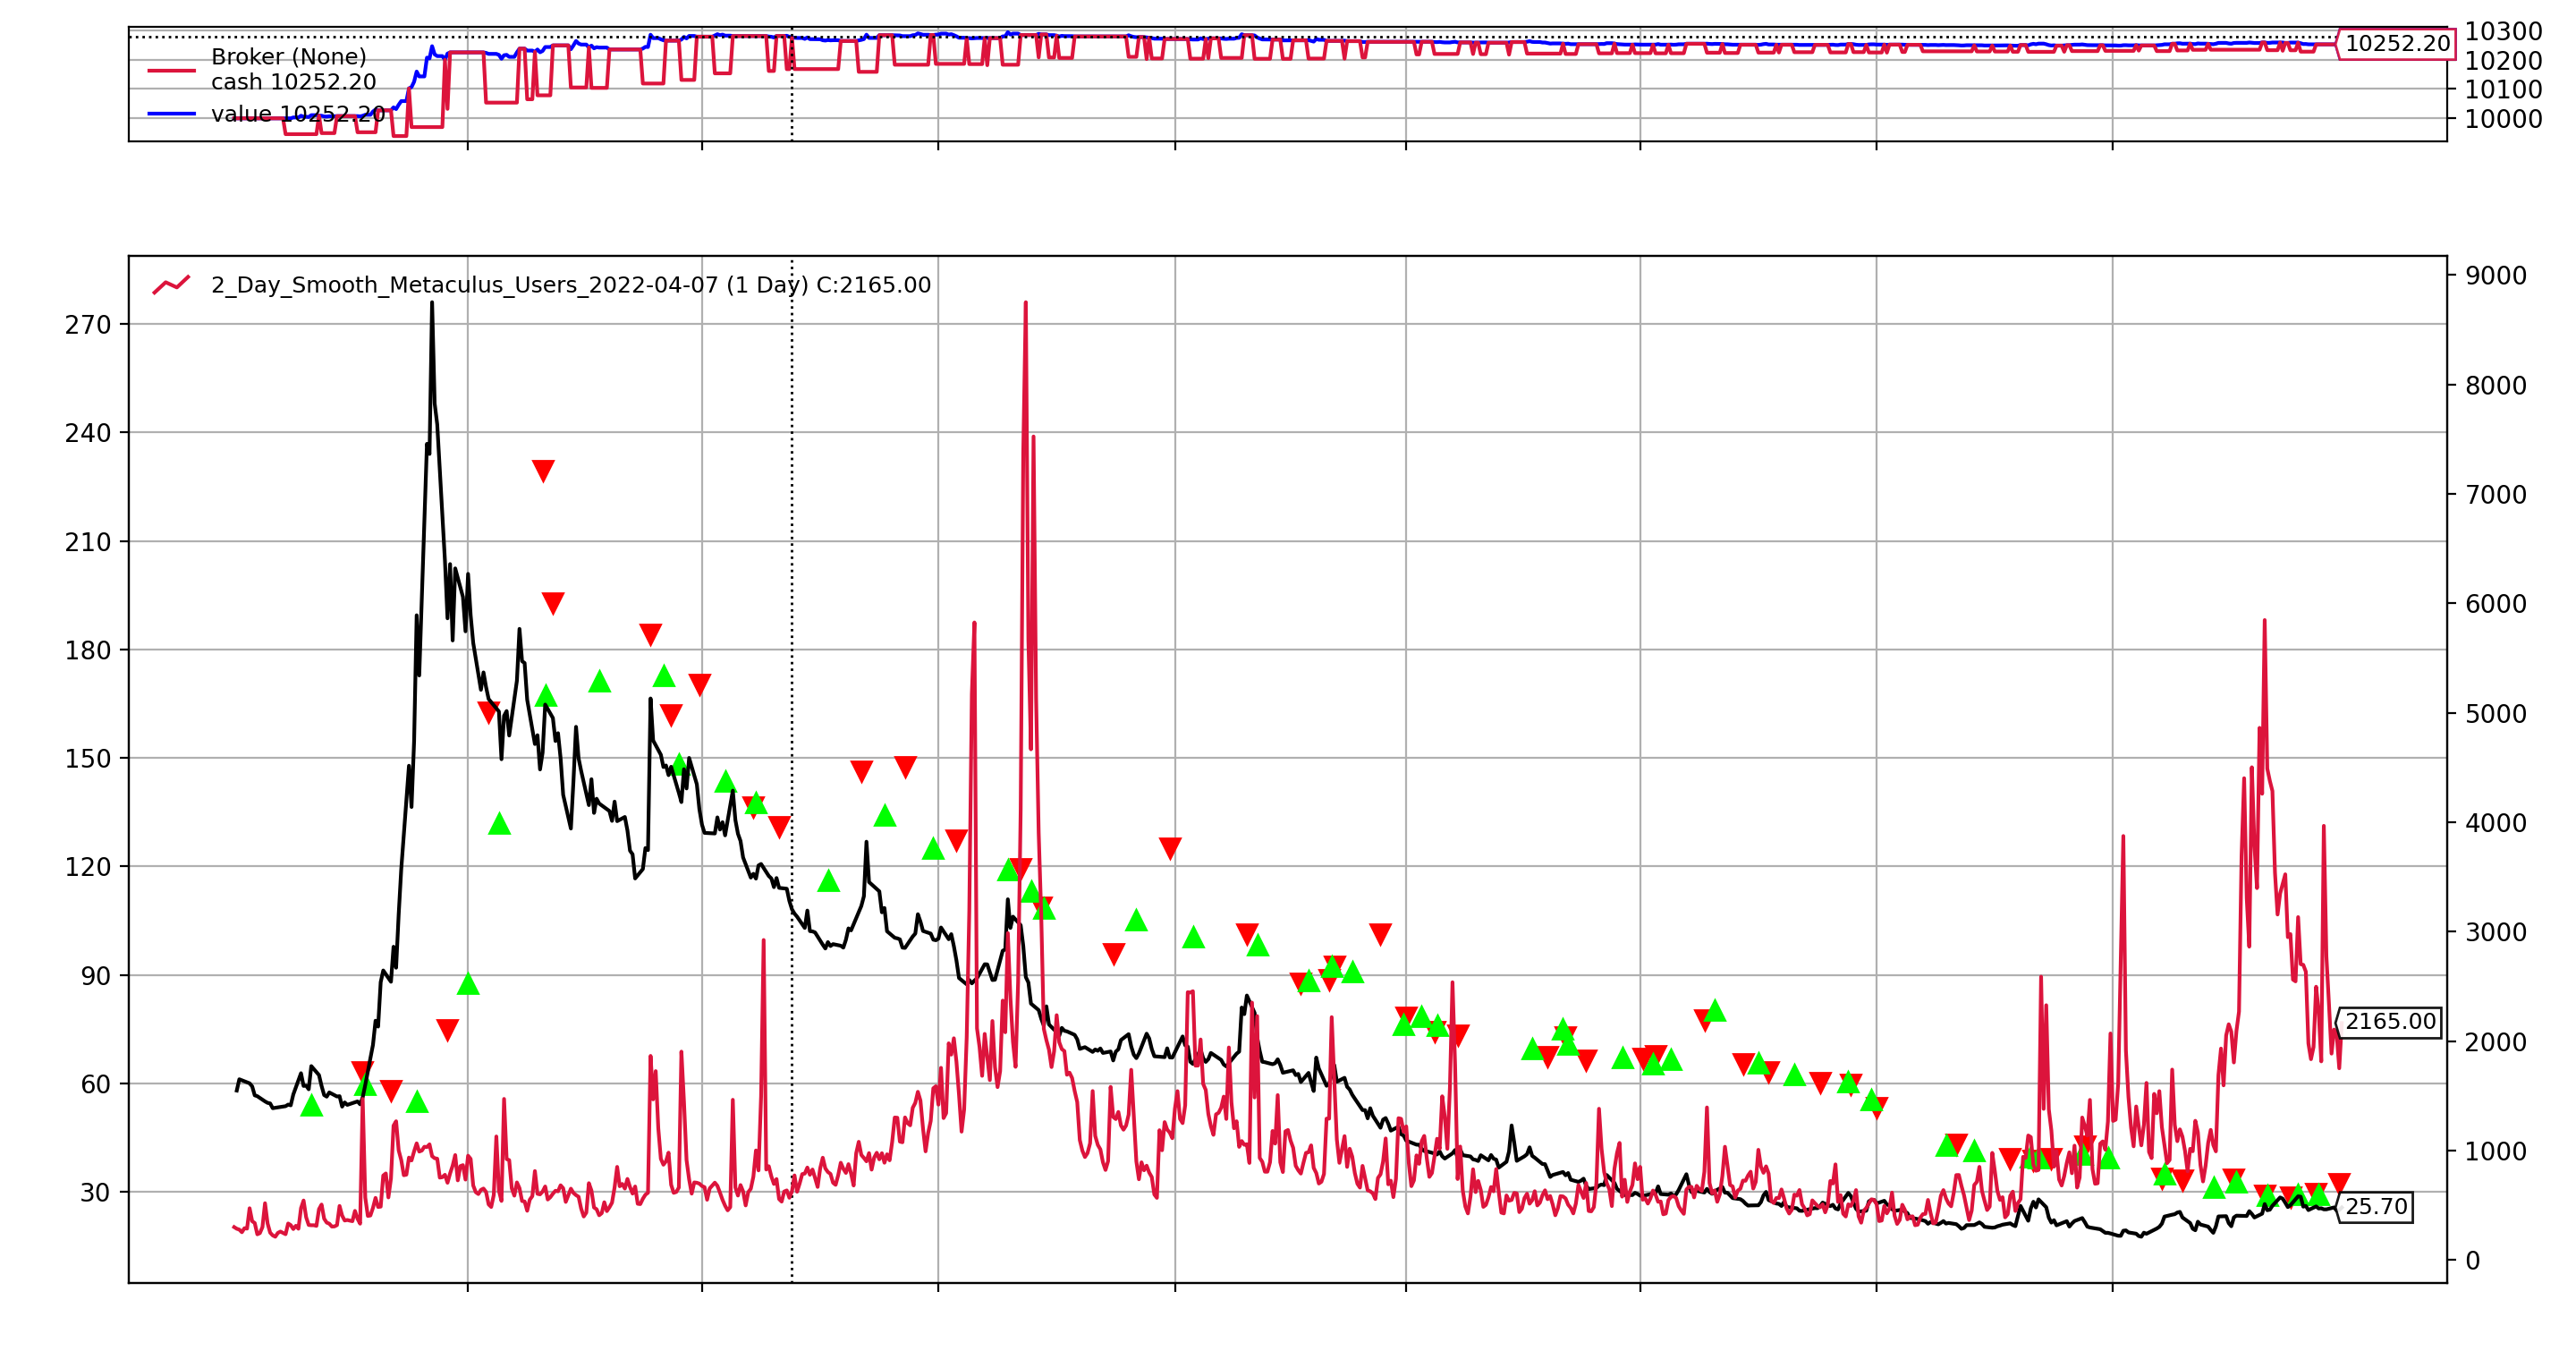
\includegraphics[width=\textwidth]{Metaculus_Lead_VXX.png}
    \caption{VXX and Metaculus Trading Plot}
\end{figure}
            
\begin{figure}[H]
    \centering
    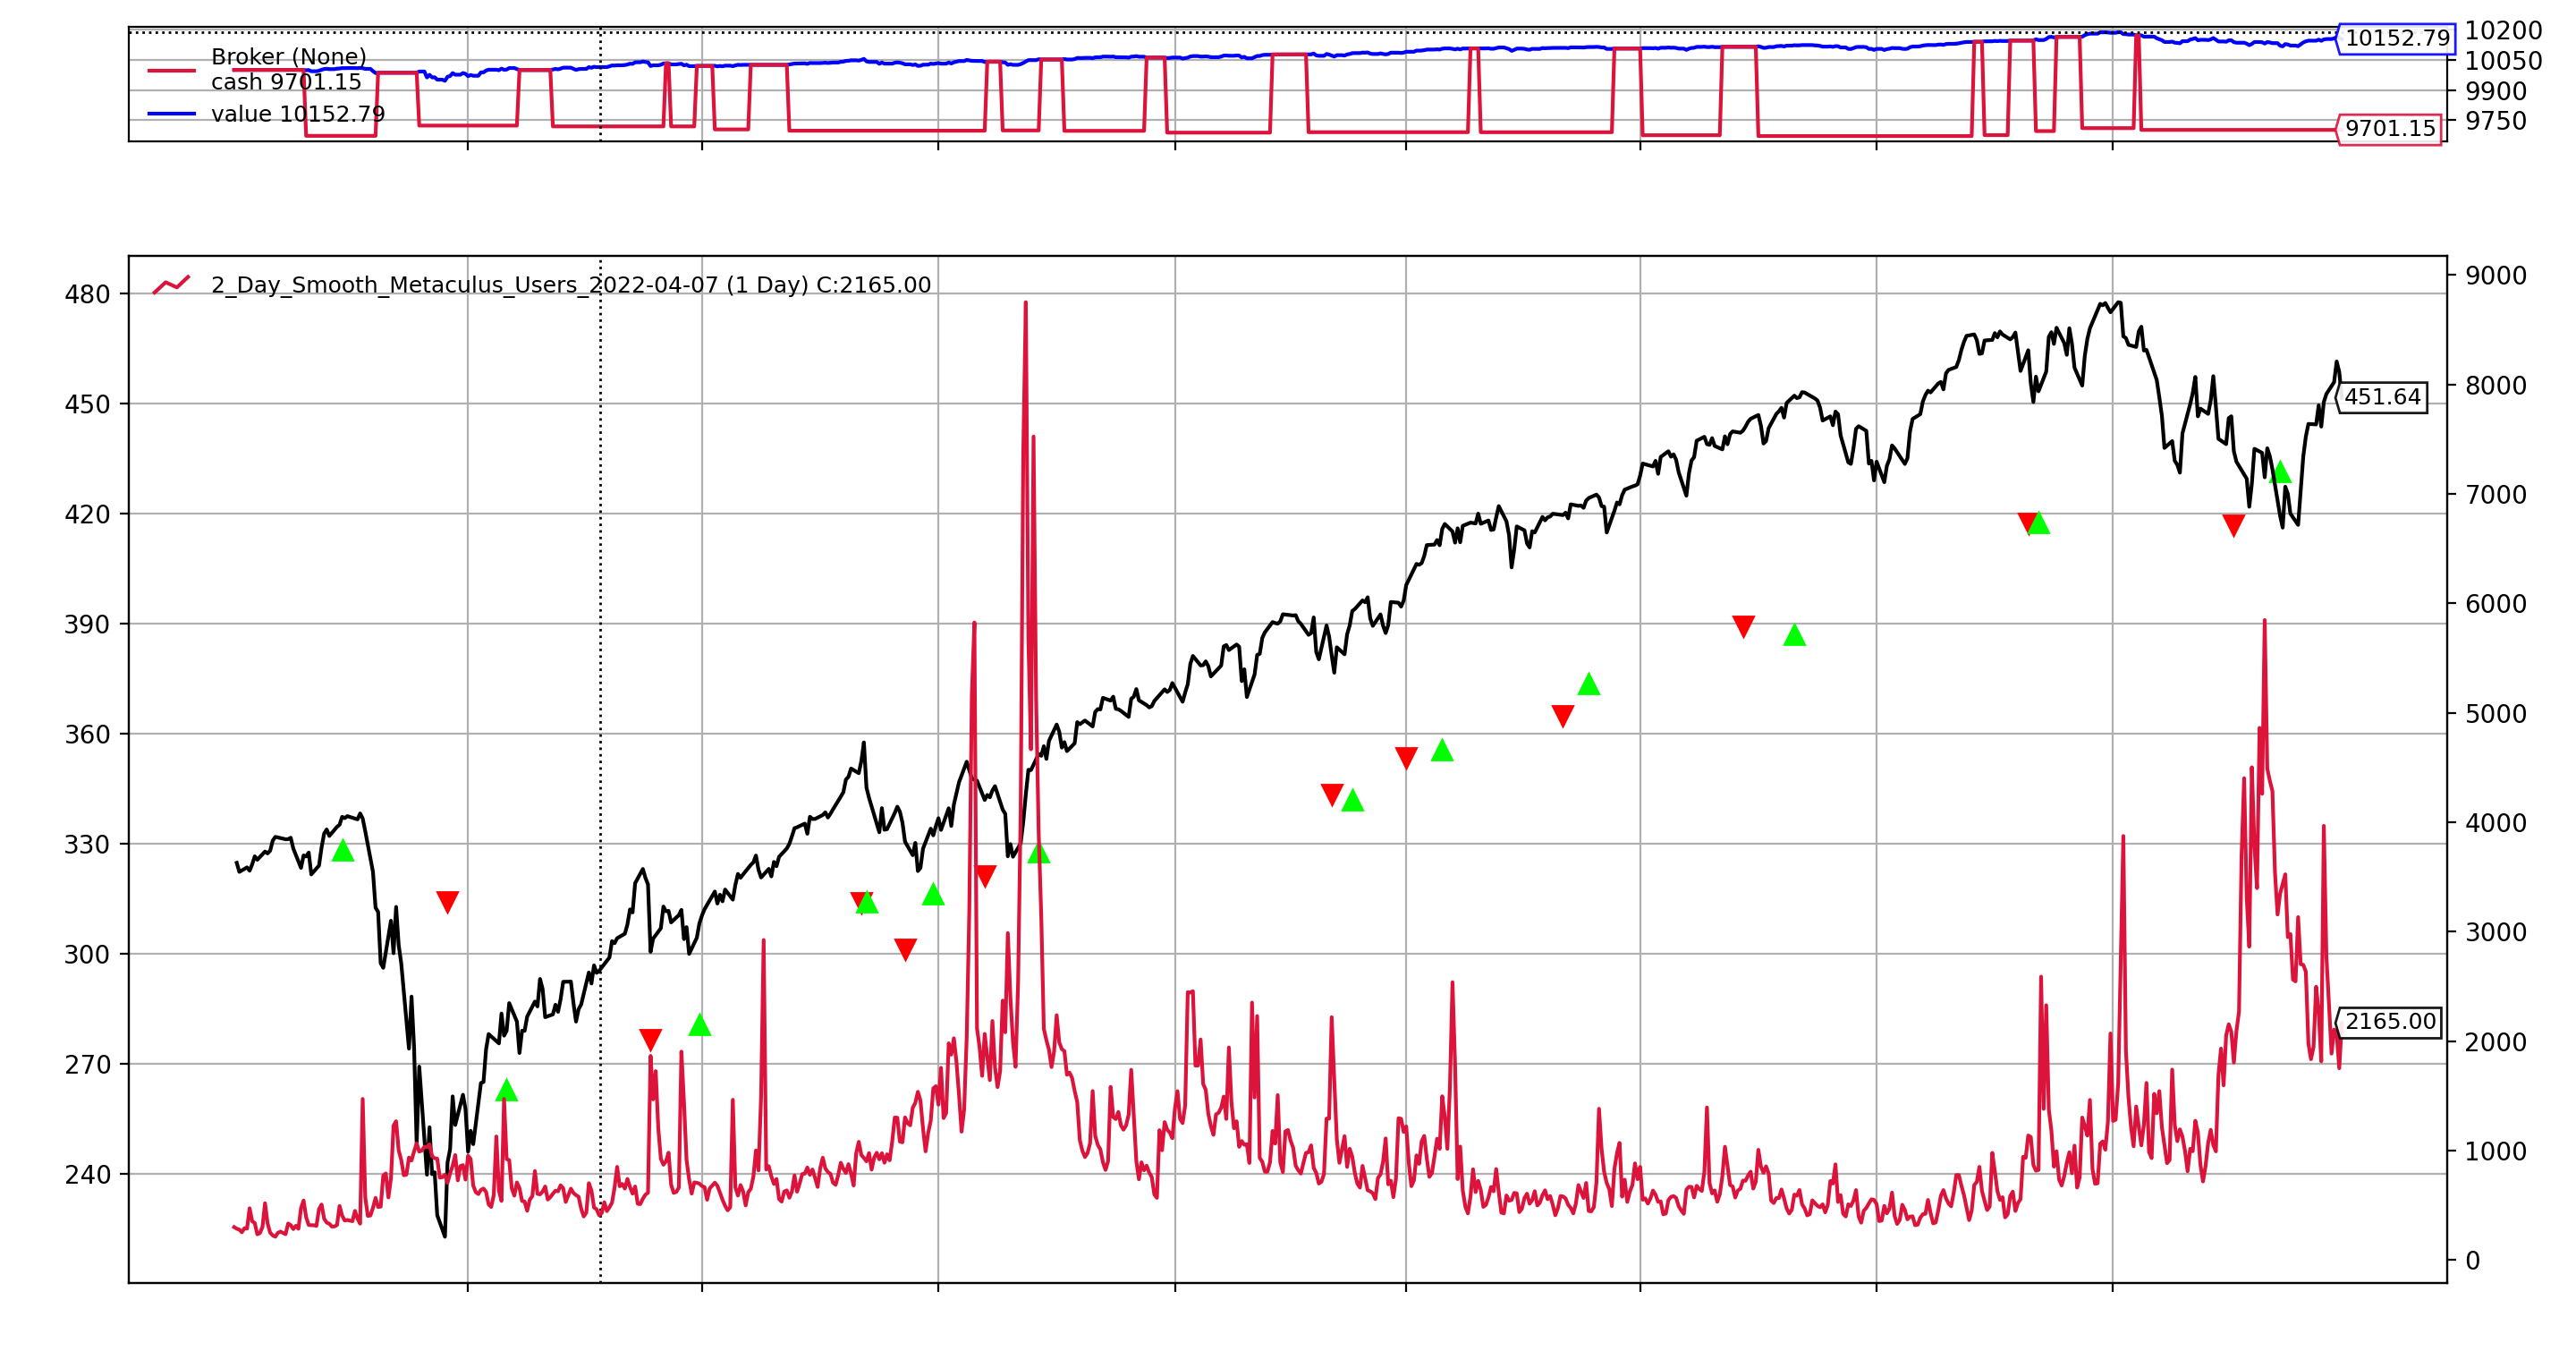
\includegraphics[width=\textwidth]{Metaculus_Lead_SPY.png}
    \caption{SPY and Metaculus Trading Plot}
\end{figure}

\end{document}